\documentclass[12pt,letterpaper]{article}

\RequirePackage{xcolor}
\definecolor{tecAzul}{cmyk}{1,0.91,0.33,0.25} % según manual de imagen 2016
\definecolor{tecRojo}{cmyk}{0,0.9,0.86,0}     % según manual de imagen 2016

\renewcommand{\familydefault}{\sfdefault}
\usepackage{amsmath} % for the equation* environment
\usepackage{mwe}
\usepackage{graphicx}
\usepackage[spanish]{babel}
\usepackage{multirow}
\usepackage{titlesec}
\titleformat*{\section}%
{\normalfont\Large\bfseries\color{tecAzul}}
\titleformat*{\subsection}%
{\normalfont\large\bfseries\color{tecAzul}}


\usepackage[tmargin=2cm,bmargin=2cm,lmargin=2.5cm,rmargin=2.5cm]{geometry}
\usepackage{textpos}
\usepackage{tikz}
\usepackage{pgfplots}
\usepackage{pgf}

\usepackage[margin=1cm]{caption}

\usepackage{hyperref}

%
% paragraph layout
%
\parindent0em                           % indentation width of first line
\parskip1.3ex                           % space between paragraphs


\newcommand{\EstudianteA}{David F. Duarte Sánchez}

\pgfplotsset{compat=1.17}



\usepackage{listings}
\usepackage{xcolor}

\definecolor{codegreen}{rgb}{0,0.6,0}
\definecolor{codegray}{rgb}{0.5,0.5,0.5}
\definecolor{codepurple}{rgb}{0.58,0,0.82}
\definecolor{backcolour}{rgb}{0.95,0.95,0.92}

\lstdefinestyle{mystyle}{
    backgroundcolor=\color{backcolour},   
    commentstyle=\color{codegreen},
    keywordstyle=\color{magenta},
    numberstyle=\tiny\color{codegray},
    stringstyle=\color{codepurple},
    basicstyle=\ttfamily\footnotesize,
    breakatwhitespace=false,         
    breaklines=true,                 
    captionpos=b,                    
    keepspaces=true,                 
    numbers=left,                    
    numbersep=5pt,                  
    showspaces=false,                
    showstringspaces=false,
    showtabs=false,                  
    tabsize=2
}

\lstset{style=mystyle}



\begin{document}
	
\graphicspath{{./}{./fig/}}

%-------------------------- Title section -------------------------------------%

%
\begin{textblock}{10}[0,0](-0.5,0)
	\large Escuela de Ingeniería Electrónica \\ 
	EL5617 Trabajo Final de Graduación \\
\end{textblock}

%
\begin{textblock}{10}[0,0](2.6,-0.35)
	\begin{flushright}
		
\includegraphics[scale=0.8]{Firma_TEC-4.pdf}
	\end{flushright}
\end{textblock}

%% Title %%
\begin{center}
	\vspace{70mm}
	{\large\color{tecRojo} Trabajo Final de Graduación}
	\par\vspace{8mm}
	{\Large\bf\color{tecAzul}{Bitácora de Trabajo - Entrega 1}}
	\par\vspace{100mm}
	{{\EstudianteA \\ II Semestre 2024} 
	\vspace{8mm}}
\end{center}

\newpage
%------------------------------------------------------------------------------%

\renewcommand{\baselinestretch}{1.1}    % line spacing

%------------------------------------------------------------------------------%

\section{Semana 5}
\subsection{Corrección de anteproyecto}

\bf{Fecha de trabajo:} 29/07/2024.\\
\bf{Objetivo:} Corrección de observaciones realizadas al anteproyecto.

% Please add the following required packages to your document preamble:
% \usepackage{graphicx}
\begin{table}[h!]
    \label{tab:my-table}
    \resizebox{\textwidth}{!}{%
    \begin{tabular}{|l|}
    \hline
    \hline
    \multicolumn{1}{|c|}{Reporte de   actividades} \\ \hline
    \hline
    - Reestructuración de las secciones del anteproyecto, ya que en la lectura   \\ 
    de los párrafos se perdía la noción de lo que se deseaba transmitir al lector. Se habla con el          \\ 
    profesor asesor y el mismo recomienda realizar mapas conceptuales con el objetivo de                    \\ 
    llevar un mejor orden de ideas.                                                                         \\\hline
    - Corrección de formato del anteproyecto usando la plantilla proporcionada por el   \\
    profesor Pablo Alvarado Moya, esto con el fin de cumplir con las normas de margenes  solicitados \\
    en el curso.\\  \hline
    - Ampliar sobre el contexto del proyecto, para que el lector pueda comprender con mas facilidad el \\
    trasfondo del proyecto y a que se dedica el laboratorio en el cual se esta desarrollando el mismo. \\ \hline\hline
    
    \hline
    \multicolumn{1}{|c|}{Productos obtenidos} \\ \hline\hline
    Se realizaron los mapas conceptuales  que se pueden observar en las Figuras \ref{fig:Entorno} y \ref{fig:definicion} con el objetivo \\ 
    de mejorar el flujo de ideas para las secciones denominadas: Entorno del proyecto y Definición del problema. \\ \hline
    Tomando en cuenta el formato de la primera versión del anteproyecto se realizaron algunos cambios, el primero \\
    de ellos fue migrar el mismo a LaTeX haciendo uso de visual studio code, esto con el fin de reducir los tiempos \\
    de compilación y la dependencia de una conexión a internet para avanzar el proyecto.\\ \hline
    Se ampliaron las referencias bibliográficas usando las siguientes fuentes que no se contenían en la primera \\
    entrega de este anteproyecto \cite{bai2023vision} ,\cite{bitlmal2024guidance}, \cite{chai2021review}, \cite{hewing2023enhancing} y \cite{karimi2021guidance}. Además de esto, se utilizo parte del contenido presente \\
    en estas referencias para dar una mejor estructura a los párrafos e intentar que las ideas expuestas fueran \\ 
    mas consistentes. \\ \hline 
    
    
    \end{tabular}%
    }
    \end{table}

    \begin{figure}[h!]
        \centering
        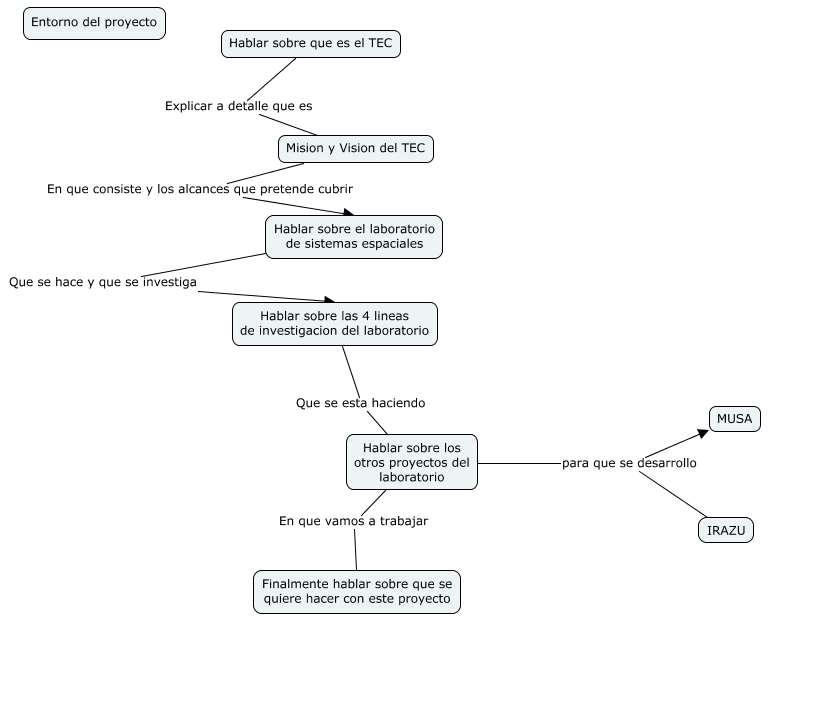
\includegraphics[width=0.8\textwidth]{Mapas conceptuales por seccion del anteproyecto/Diagrama_Entorno_del proyecto.png}
        \caption{Entorno del proyecto}
        \label{fig:Entorno}
      \end{figure}
      \newpage

      \begin{figure}[h!]
        \centering
        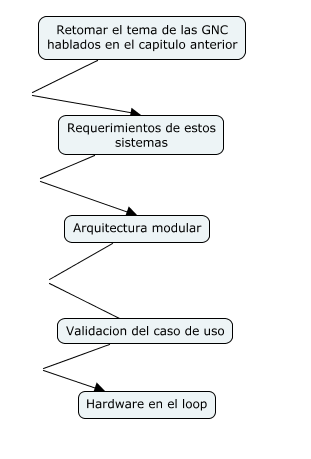
\includegraphics[width=0.3\textwidth]{Mapas conceptuales por seccion del anteproyecto/Diagrama_Entorno.png}
        \caption{Definición del problema}
        \label{fig:definicion}
      \end{figure}


      \bf{Fecha de trabajo:} 8/08/2024.\\
      \bf{Objetivo:} Corrección de observaciones realizadas al anteproyecto.


      \begin{table}[h!]
          \label{tab:my-table}
          \resizebox{\textwidth}{!}{
          \begin{tabular}{|l|}
          \hline
          \hline
          \multicolumn{1}{|c|}{Reporte de   actividades} \\ \hline
          \hline
          - Agrega el nombre del software propietario a utilizar a la Alternativa 1 : Matlab y Simulink.        \\ \hline
          - Se establece el día en el cual se tendrán las reuniones semanales, se selecciona el mismo como los  \\
          días Jueves a las 10:00 am\\ \hline
          - Se propone el avance de los primeros capítulos del anteproyecto, así como el trabajar en una presentación \\
          breve del anteproyecto para el caso de los profesores lectores así como al profesor asesor del proyecto \\
          esto con el fin de mantener a los profesores lectores al tanto del objetivo y avances del proyecto. \\ \hline
          - Planteamiento de la estructura a manejar para los capítulos de la tesis, el mismo se enfocara en dividir los \\
          capítulos en tres partes, en la primera sub-sección del capitulo se explicaran los conceptos que se abarcaran en \\ 
          el mismo, seguido de esto se realiza una revisión de literatura general relacionada al tema de investigación \\
          finalmente se realiza una investigación del estado del arte de los últimos 2 años, con el fin de proporcionar\\
          al lector el panorama mas completo sobre el impacto que tendrá la solución propuesta\\ \hline
          - Se deberá de investigar sobre como se traduce el código para los sistemas embebidos actualmente y en que se \\
          diferencia el sistema actual al que se desea realizar en este proyecto.\\ \hline \hline
          
          \multicolumn{1}{|c|}{Productos obtenidos}                            \\ \hline\hline
          Se especifica para la Alternativa 1 el software a utilizar con el fin de delimitar la solución a un marco de trabajo.\\ 
          También se genera una reunión recurrente desde la fecha de la reunión hasta el final del semestre y la entrega de \\
          las bitácoras de forma semanal, esto con el fin de revisar periódicamente los avances del proyecto y poder cumplir \\
          con la ruta critica plateada en el diagrama de Gantt. Seguido de esto se plantea la generación de mapas conceptuales \\
          para poder verificar la estructura de los párrafos y respetar la estructura de capitulo sugerida por el profesor asesor. \\
          Además se comienza una breve investigación con el fin de investigar un poco sobre la traducción o generación de código \\
          para sistemas embebidos \cite{mathworks_code_generation}, \cite{suarez2018metodologias}, \cite{galeano2009programacion} y \cite{osio2007optimizacion} \\
          \hline
          \end{tabular}
            }
          \end{table}

\bibliography{bibliografia_consultada}
\bibliographystyle{plain}
\end{document}